\subsection{For Any Cosine-Based Loss, the Output Gradient Is Orthogonal to the Encoder Output}

Let the embedding $q$ produced by the encoder participate in the loss only via cosine similarities with other embeddings generated by the two-tower model. Then the loss can be written as
\begin{align}
\mathcal L \,=\, F\bigl(\cos(q,k_1),\dots,\cos(q,k_r)\bigr).
\end{align}
And its gradient with respect to $q$ is
\begin{align}
\nabla_q\mathcal L \,=\, \sum_{s=1}^{r} \frac{\partial F}{\partial \cos(q,k_s)}\, \nabla_q \cos(q,k_s). \label{eq:grad-cos-loss}
\end{align}
Here the derivative of the loss with respect to a cosine is a scalar. I can say that the loss gradient with respect to $q$ is orthogonal to $q$ if
\begin{align}
\langle q,\nabla_q\mathcal L \rangle \,=\, 0.
\end{align}
Therefore,
\begin{equation}
\begin{aligned}
\langle q,\nabla_q\mathcal L \rangle 
&= \sum_{s=1}^{r} \frac{\partial F}{\partial \cos(q,k_s)}\, \langle q,\nabla_q \cos(q,k_s) \rangle \\
&= 0.
\end{aligned}
\end{equation}
Here I used lemma in Appendix~\ref{app:cos-orth-lemma}, which states that $\langle q, \nabla_q \cos(q,\ast) \rangle = 0$.
Hence $q_i \perp g_i$ for any cosine loss. Consequently, if $\Delta q_i \parallel g_i$, then $q_i \perp \Delta q_i$: during training the embedding moves orthogonally:

\begin{figure}[!htbp]
\centering
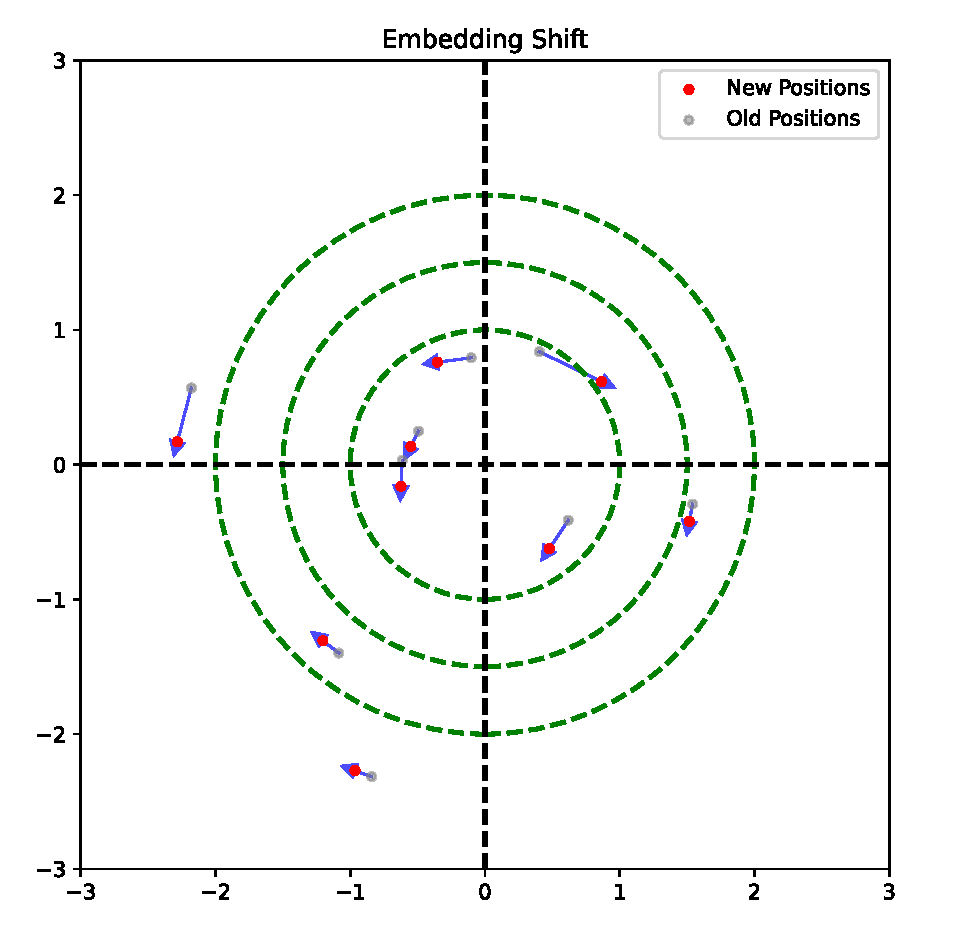
\includegraphics[width=.95\columnwidth]{../draft_materials/figure_2_paper.pdf}
\caption{Orthogonal movement during training.}
\label{fig:cos-orth}
\end{figure}

